\section{Results}

\subsection{Kernels}

Table~\ref{tab:kernels} gives test accuracy pooled over the five shares, \N{n_splits_all} splits per row, and Fig.~\ref{fig:kernel} shows the 80/20 case. On each of the three problems that are not linearly separable, the Gaussian kernel has the highest mean: \N{gauss_p2_mean} on Problem 2, \N{gauss_p3_mean} on Problem 3, and \N{gauss_p4_mean} on Problem 4. Averaged over the three problems, it scores \N{gauss_p234}, against \N{dot_p234} for the dot product, \N{d2_p234} for degree 2, and \N{d3_p234} for degree 3. The 95\% interval of each Gaussian mean is within \N{gauss_ci_halfwidth_ub} of it. A single split can land well away from the mean: the 2.5th and 97.5th percentiles of the Gaussian's single splits are \N{gauss_p3_rlo} and \N{gauss_p3_rhi} on Problems 3 and 4, and \N{gauss_p2_rlo} and \N{gauss_p2_rhi} on Problem 2.

\begin{figure*}[t]
\centering
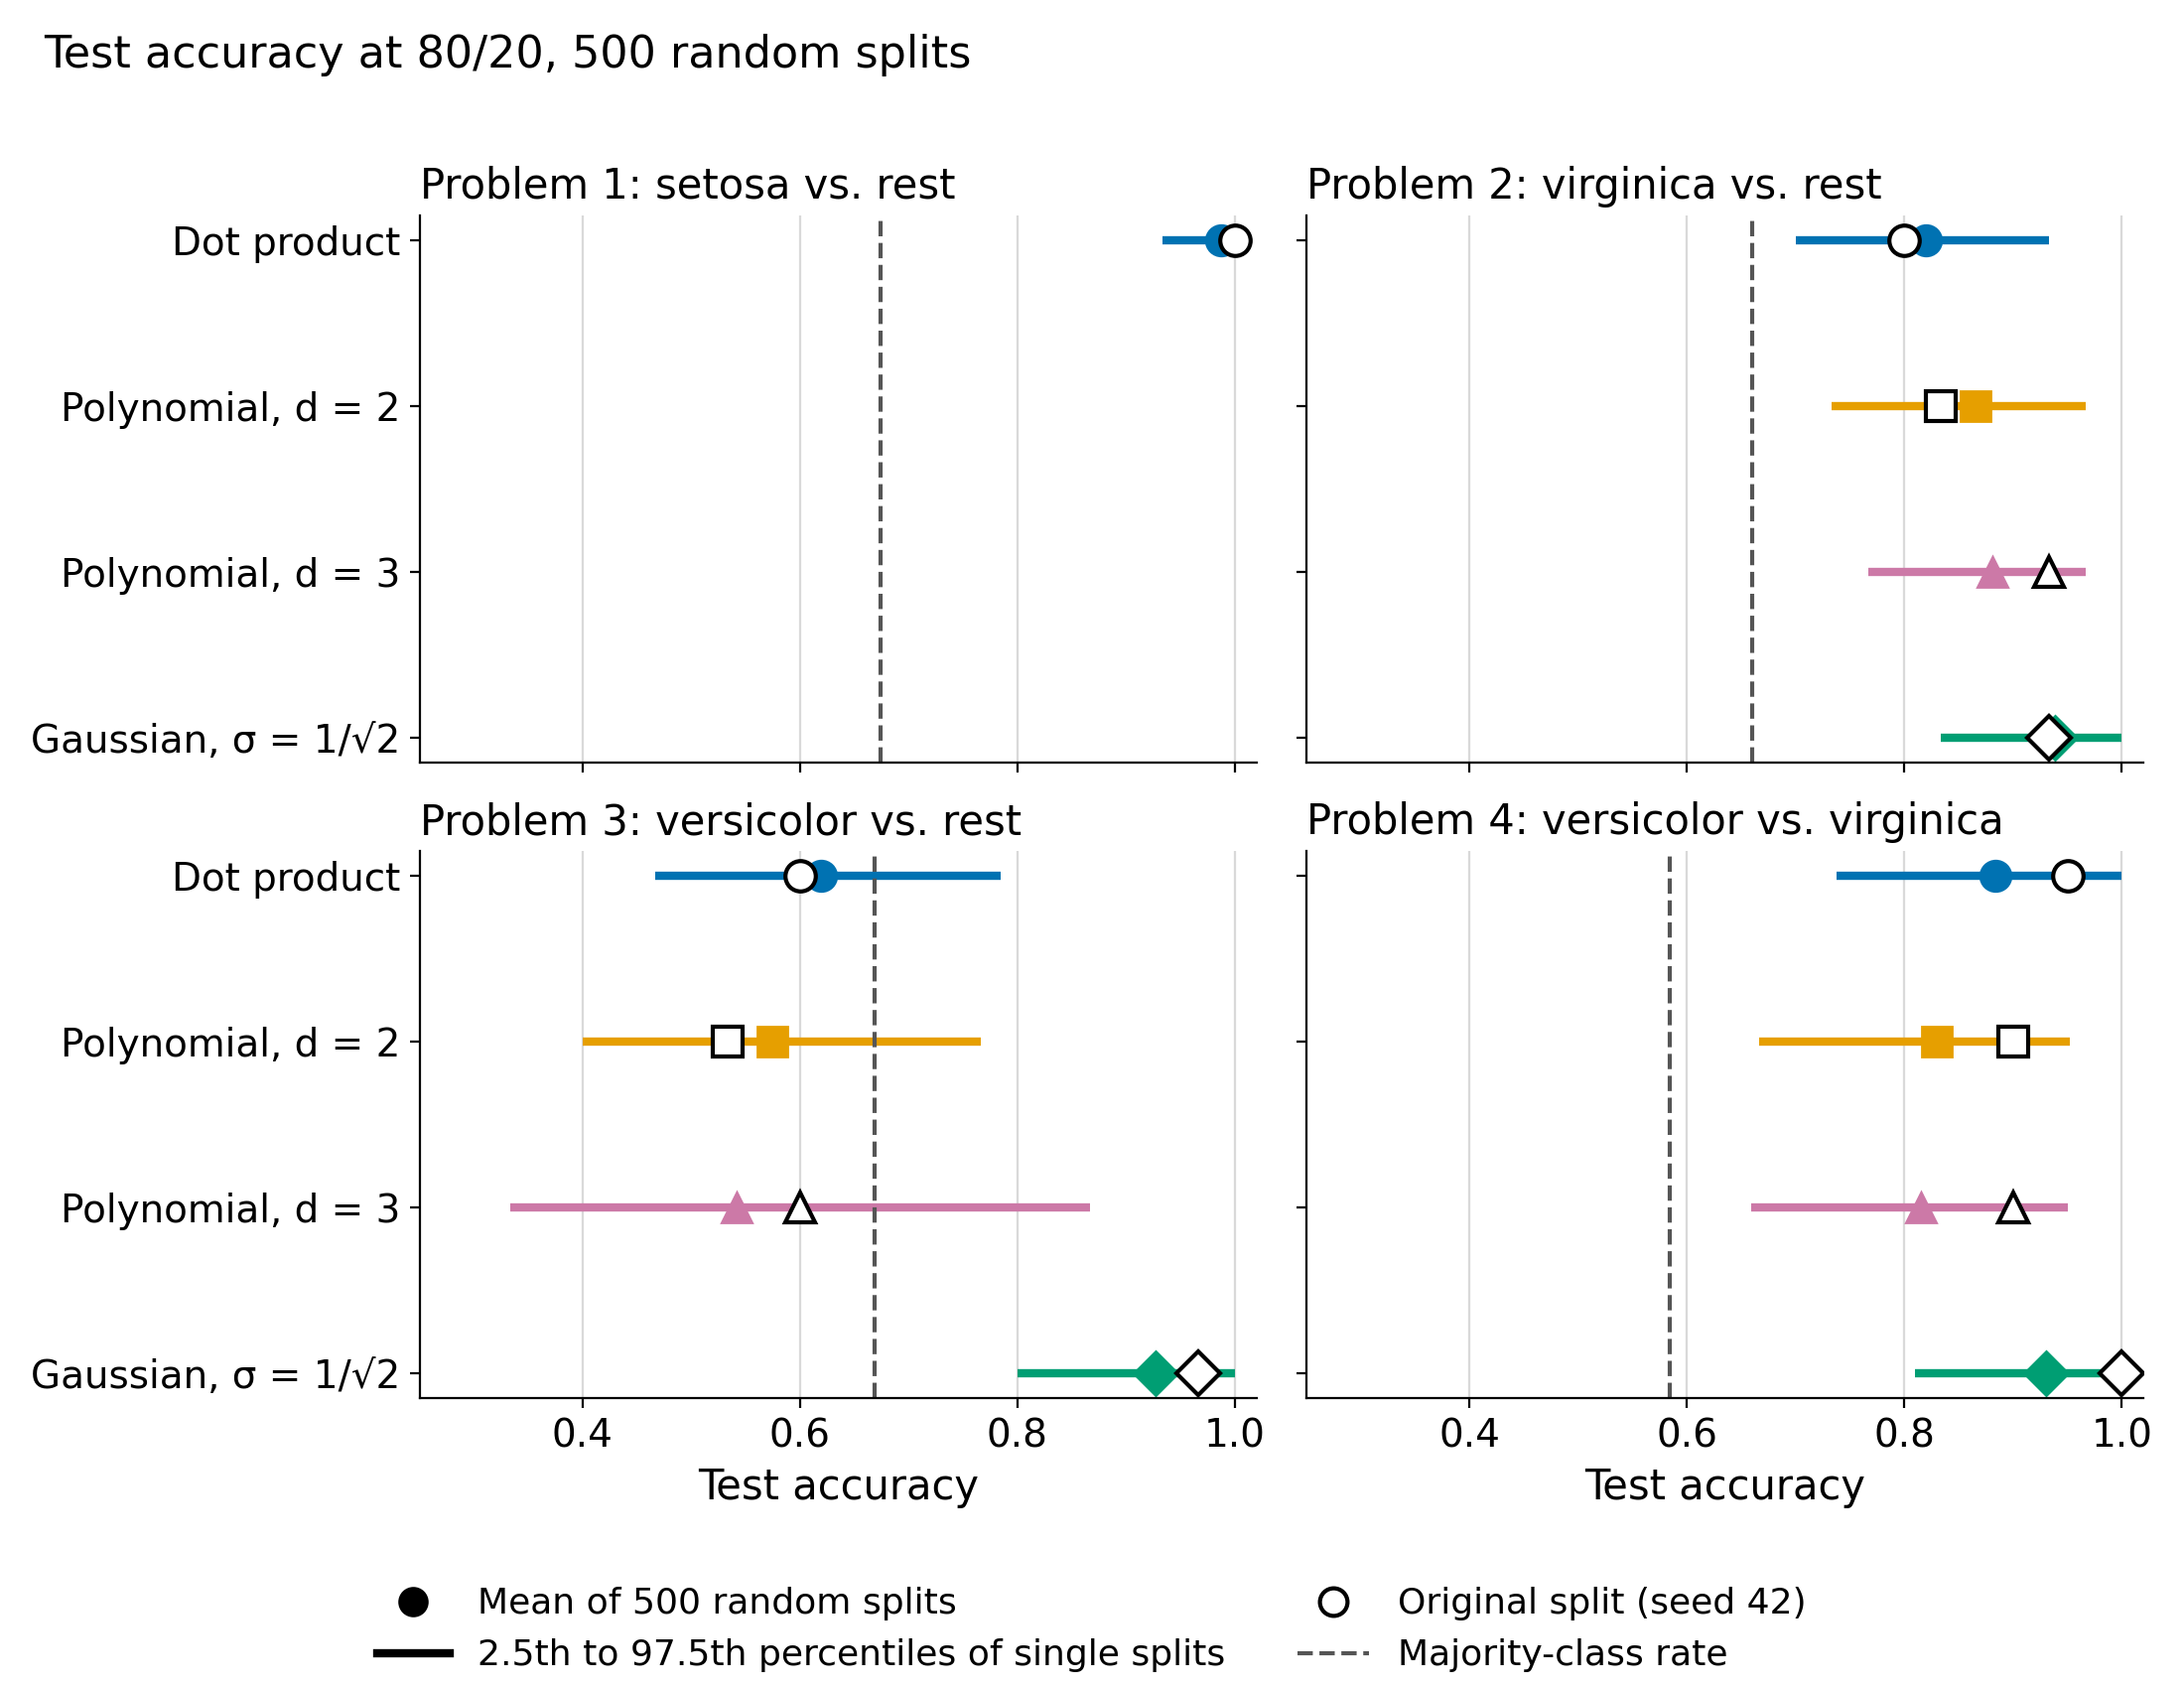
\includegraphics[width=0.7\textwidth]{../repeated_splits/repeated_split_by_kernel.png}
\caption{Test accuracy at 80/20 over \N{n_splits_ratio} random splits, with \N{test_n_r80} test flowers on Problems 1 to 3 and fewer on Problem 4, which leaves out setosa. Filled markers are means, bars span the 2.5th to 97.5th percentiles of single splits, open markers are the original split (seed 42), and the dashed line is the mean majority-class rate.}
\label{fig:kernel}
\end{figure*}

\begin{table*}[t]
\caption{Test accuracy by problem and kernel, pooled over the five training shares (\N{n_splits_all} splits per row). The 95\% CI of the mean is computed from the \N{n_splits_ratio} per-seed means (each the mean of one seed's five splits) and covers the choice of splits only. ``Original'' is the mean of the five original single-split runs.}
\label{tab:kernels}
\centering
\begin{tabular}{@{}clcccc@{}}
\toprule
Prob. & Kernel & Mean & 95\% CI of mean & 2.5th to 97.5th percentiles of splits & Original \\
\midrule
1 & Dot product & 0.987 & 0.986--0.988 & 0.933--1.000 & 1.000 \\
\midrule
2 & Dot product & 0.821 & 0.816--0.825 & 0.667--0.933 & 0.788 \\
 & Polynomial, $d=2$ & 0.865 & 0.861--0.869 & 0.733--1.000 & 0.828 \\
 & Polynomial, $d=3$ & 0.880 & 0.876--0.883 & 0.767--1.000 & 0.909 \\
 & Gaussian & \textbf{0.938} & 0.935--0.941 & 0.842--1.000 & 0.951 \\
\midrule
3 & Dot product & 0.622 & 0.617--0.627 & 0.467--0.800 & 0.674 \\
 & Polynomial, $d=2$ & 0.574 & 0.569--0.580 & 0.400--0.747 & 0.628 \\
 & Polynomial, $d=3$ & 0.546 & 0.539--0.552 & 0.333--0.860 & 0.555 \\
 & Gaussian & \textbf{0.926} & 0.923--0.929 & 0.800--1.000 & 0.966 \\
\midrule
4 & Dot product & 0.881 & 0.877--0.886 & 0.738--1.000 & 0.924 \\
 & Polynomial, $d=2$ & 0.832 & 0.827--0.837 & 0.667--1.000 & 0.875 \\
 & Polynomial, $d=3$ & 0.817 & 0.812--0.821 & 0.644--1.000 & 0.859 \\
 & Gaussian & \textbf{0.929} & 0.925--0.932 & 0.800--1.000 & 0.987 \\
\bottomrule
\end{tabular}

\end{table*}

The lead holds on most single splits. On the same split, the Gaussian is at least as accurate as the best other kernel in \N{gauss_ge_p2}\%, \N{gauss_ge_p3}\%, and \N{gauss_ge_p4}\% of the \N{n_splits_all} splits on Problems 2, 3, and 4, and strictly more accurate in \N{gauss_gt_p2}\%, \N{gauss_gt_p3}\%, and \N{gauss_gt_p4}\%. Its mean margin over the best other kernel is \N{gauss_margin_p2}, \N{gauss_margin_p3}, and \N{gauss_margin_p4}.

Problem 3 separates the kernels most. Versicolor lies between setosa and virginica, so the ``rest'' class has one part on each side of it, and the mean of ``rest'' falls near versicolor. A rule that compares the class means of the raw measurements, as the dot product does, has little to work with there. The dot-product, degree-2, and degree-3 kernels average \N{dot_p3_mean}, \N{d2_p3_mean}, and \N{d3_p3_mean}, all below the majority-class rate of \N{maj_p3}, which is about what always predicting ``rest'' scores. The Gaussian averages \N{gauss_p3_mean}. This is consistent with its window ($\sigma \approx 0.71$) being small next to the distances between the mean measurements of neighboring species (\N{dist_set_ver}~cm for setosa and versicolor, \N{dist_ver_vir}~cm for versicolor and virginica), which keeps the two parts of ``rest'' apart.

Problem 1 is easy, but the rule is not perfect on it. Over random splits, the dot product averages \N{dot_p1_mean} on the test sets. On the original splits, it classified every test flower correctly, but its training accuracy was \N{p1_orig_train_min} to \N{p1_orig_train_max}: in each original split, it misclassified one versicolor flower of the training set, and two at 90/10, even though the classes are linearly separable. Those flowers are nearest their own species' mean, but the rule compares the setosa mean with the mean of versicolor and virginica combined, which virginica pulls away from them, and they lie nearer the setosa mean. With standardized features, the dot product classifies every Problem 1 flower correctly, in training and test sets alike (test sets in Table~\ref{tab:std}).

The polynomial kernels underfit and show little sign of overfitting. Over random splits, their training accuracy is as low as their test accuracy: the two means differ by at most \N{train_test_gap_max} for every problem--kernel pair except the degree-3 kernel on Problem 3 (\N{d3_p3_train} on training sets against \N{d3_p3_mean} on test sets). Nothing is tuned, and the only quantities taken from the training set are the two class means in feature space and $b$, so these low accuracies are consistent with underfitting on the raw measurements. The degree-3 gap on Problem 3 is the exception, likely because each training flower counts toward its own class mean, which favors it on the training set.

\subsection{Training share}

Figure~\ref{fig:ratio} shows each kernel's mean over Problems 2 to 4 by training share. Averaged over the 13 problem--kernel pairs, mean test accuracy is \N{all13d_r90}, \N{all13d_r80}, \N{all13d_r70}, \N{all13d_r60}, and \N{all13d_r50} at 90/10, 80/20, 70/30, 60/40, and 50/50. The Gaussian's mean over Problems 2 to 4 is \N{gauss234d_r90}, \N{gauss234d_r80}, \N{gauss234d_r70}, \N{gauss234d_r60}, and \N{gauss234d_r50}. The training share between 50\% and 90\% has little effect on the mean test accuracy averaged over the 13 pairs: the largest difference between the observed means is under \N{all13_span_ub}. Single pairs move more, by up to \N{cfg_share_span_max} across the five shares. That fits a rule built from class means, which \N{train_n_r50} training flowers (the 50/50 case on Problems 1 to 3) may already estimate well; this explanation is consistent with the result but was not tested. The kernel matters far more than the share: on Problem 3, the means of the best and worst kernels differ by \N{p3_spread}.

\begin{figure}[t]
\centering
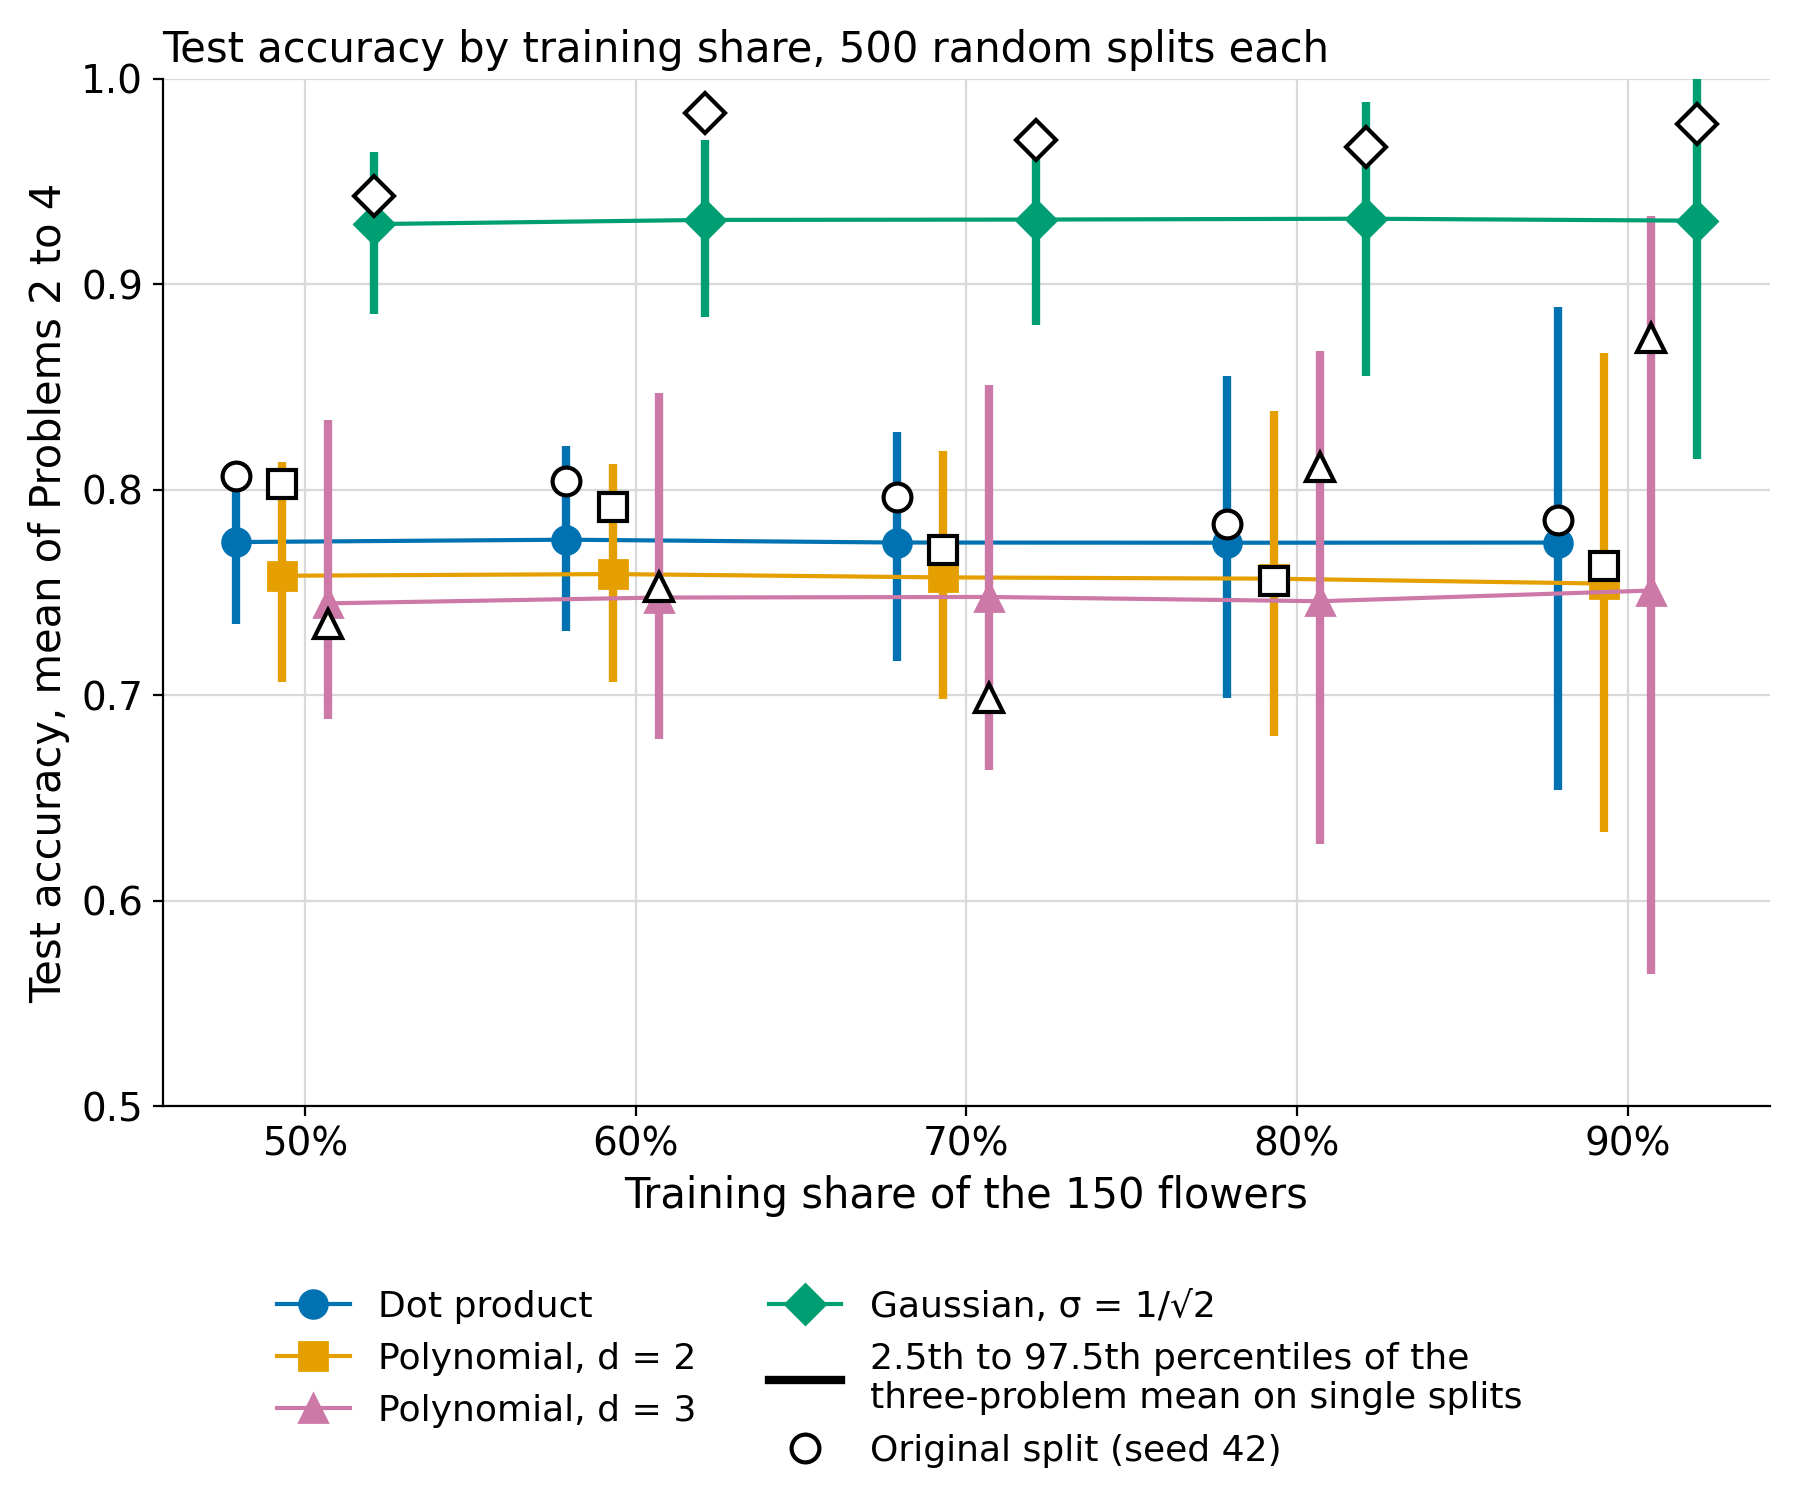
\includegraphics[width=\columnwidth]{../repeated_splits/repeated_split_by_ratio.png}
\caption{Mean test accuracy over Problems 2 to 4 by training share, \N{n_splits_ratio} random splits per share. Bars span the 2.5th to 97.5th percentiles of the three-problem mean on single splits, and open markers are the original split.}
\label{fig:ratio}
\end{figure}

The original splits suggested otherwise. Their mean over the 13 problem--kernel pairs ranged from \N{orig13_min} to \N{orig13_max} across shares, a spread of \N{orig13_span}, with no steady trend. The five test sets are nested, so the five values are not independent, and the spread reflects which flowers each test set happened to contain. The original split scored above the mean of its \N{n_splits_ratio} random splits in \N{orig_above_n} of the \N{orig_total_n} problem--kernel--share runs, and \N{orig_mean65} on average against \N{rand_mean65}. For the Gaussian on Problems 2 to 4, it scored \N{gauss_p234_orig} against \N{gauss_p234}. The original draw was a favorable one, and its headline accuracies are higher than random splits give.

\subsection{Standardized features}

The dot-product and polynomial kernels depend on the origin and the units of the features, which here are raw centimeters. Table~\ref{tab:std} repeats the evaluation on the same splits with standardized features. Standardizing changes one result a lot. On Problem 3, the degree-2 kernel rises from \N{s_d2_p3_raw} to \N{s_d2_p3_std}, higher on \N{s_d2_p3_hi}\% of splits, and the degree-3 kernel rises from \N{s_d3_p3_raw} to \N{s_d3_p3_std}. Their training accuracy rises with it, to \N{s_d2_p3_train} and \N{s_d3_p3_train}, and mean training and test accuracy now agree within \N{s_p3_poly_gap_max}, so they still show little sign of overfitting. Standardizing also makes Problem 1 perfect: the dot product scores \N{s_dot_p1_std} on every training and test set, higher than on raw features on \N{s_dot_p1_hi}\% of splits and lower on none.

\begin{table}[t]
\caption{Test accuracy on raw and standardized features, same \N{n_splits_all} splits per row. ``Higher / lower'' is the share of splits on which standardizing raised or lowered accuracy.}
\label{tab:std}
\centering
\footnotesize
\setlength{\tabcolsep}{3pt}
\begin{tabular}{@{}clcccc@{}}
\toprule
Prob. & Kernel & Raw & Standardized & Change & Higher / lower \\
\midrule
1 & Dot product & 0.987 & 1.000 & +0.013 & 45.2\% / 0.0\% \\
\midrule
2 & Dot product & 0.821 & 0.836 & +0.016 & 52.1\% / 5.3\% \\
 & Polynomial, $d=2$ & 0.865 & 0.872 & +0.007 & 44.0\% / 32.1\% \\
 & Polynomial, $d=3$ & 0.880 & 0.881 & +0.001 & 44.2\% / 32.1\% \\
 & Gaussian & 0.938 & 0.904 & $-$0.034 & 1.8\% / 71.0\% \\
\midrule
3 & Dot product & 0.622 & 0.646 & +0.024 & 61.0\% / 19.8\% \\
 & Polynomial, $d=2$ & 0.574 & 0.853 & +0.278 & 99.7\% / $<$0.1\% \\
 & Polynomial, $d=3$ & 0.546 & 0.771 & +0.225 & 92.0\% / 5.4\% \\
 & Gaussian & 0.926 & 0.908 & $-$0.018 & 12.2\% / 50.0\% \\
\midrule
4 & Dot product & 0.881 & 0.881 & $-$0.001 & 34.3\% / 34.9\% \\
 & Polynomial, $d=2$ & 0.832 & 0.850 & +0.018 & 48.0\% / 22.0\% \\
 & Polynomial, $d=3$ & 0.817 & 0.808 & $-$0.009 & 35.8\% / 39.0\% \\
 & Gaussian & 0.929 & 0.928 & $-$0.001 & 31.3\% / 32.1\% \\
\bottomrule
\end{tabular}

\end{table}

On Problems 2 and 4, standardizing moves the dot-product and polynomial kernels by at most \N{s_p24_maxabs} either way. The Gaussian, with $\sigma = 1/\sqrt{2}$ now applied to standardized features, falls from \N{s_gauss_p2_raw} to \N{s_gauss_p2_std} on Problem 2 (lower on \N{s_gauss_p2_lo}\% of splits) and from \N{s_gauss_p3_raw} to \N{s_gauss_p3_std} on Problem 3, and barely changes on Problem 4 (\N{s_gauss_p4_raw} and \N{s_gauss_p4_std}). It still has the highest mean on Problems 2 to 4, but on Problem 3, its lead over the degree-2 kernel shrinks from \N{s_gap_p3_raw} to \N{s_gap_p3_std}. The kernel gaps in Table~\ref{tab:kernels} therefore depend partly on how the features are centered and scaled, and so does the failure of the polynomial kernels on Problem~3. Standardizing does both, and this comparison does not separate them.
